\documentclass{article}
\usepackage{tikz}
\usetikzlibrary{calc,fadings,decorations.pathreplacing}
%% helper macros

\newcommand\pgfmathsinandcos[3]{%
  \pgfmathsetmacro#1{sin(#3)}%
  \pgfmathsetmacro#2{cos(#3)}%
}
\newcommand\LongitudePlane[3][current plane]{%
  \pgfmathsinandcos\sinEl\cosEl{#2} % elevation
  \pgfmathsinandcos\sint\cost{#3} % azimuth
  \tikzset{#1/.estyle={cm={\cost,\sint*\sinEl,0,\cosEl,(0,0)}}}
}
\newcommand\LatitudePlane[3][current plane]{%
  \pgfmathsinandcos\sinEl\cosEl{#2} % elevation
  \pgfmathsinandcos\sint\cost{#3} % latitude
  \pgfmathsetmacro\yshift{\cosEl*\sint}
  \tikzset{#1/.estyle={cm={\cost,0,0,\cost*\sinEl,(0,\yshift)}}} %
}
\newcommand\DrawLongitudeCircle[2][1]{
  \LongitudePlane{\angEl}{#2}
  \tikzset{current plane/.prefix style={scale=#1}}
   % angle of ``visibility''
  \pgfmathsetmacro\angVis{atan(sin(#2)*cos(\angEl)/sin(\angEl))} %
  \draw[current plane] (\angVis:1) arc (\angVis:\angVis+180:1);
  \draw[current plane,dashed] (\angVis-180:1) arc (\angVis-180:\angVis:1);
}
\newcommand\DrawLatitudeCircle[2][1]{
  \LatitudePlane{\angEl}{#2}
  \tikzset{current plane/.prefix style={scale=#1}}
  \pgfmathsetmacro\sinVis{sin(#2)/cos(#2)*sin(\angEl)/cos(\angEl)}
  % angle of ``visibility''
  \pgfmathsetmacro\angVis{asin(min(1,max(\sinVis,-1)))}
  \draw[current plane] (\angVis:1) arc (\angVis:-\angVis-180:1);
  \draw[current plane,dashed] (180-\angVis:1) arc (180-\angVis:\angVis:1);
}

%% document-wide tikz options and styles

\tikzset{%
  >=latex, % option for nice arrows
  inner sep=0pt,%
  outer sep=2pt,%
  mark coordinate/.style={inner sep=0pt,outer sep=0pt,minimum size=3pt,
    fill=black,circle}%
}

\begin{document}

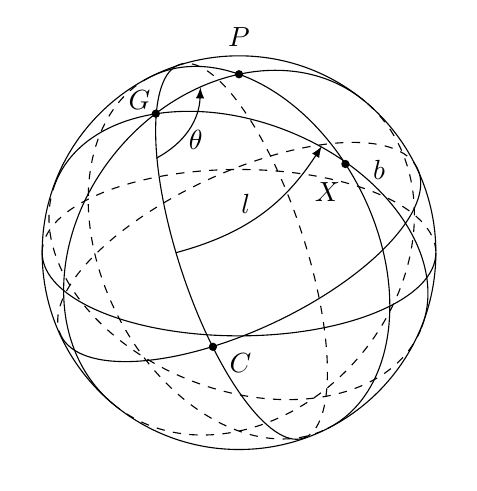
\begin{tikzpicture}

%definitions
\def\R{2.5} % sphere radius
\def\angEl{25} % elevation angle
\def\angLL{25} % elevation angle of Galactic plane
\def\angPhiX{-45} % longitude of point X
\def\angPhiGamma{-95} % longitude of point Gamma
\def\angBetaX{40} % latitude of point X
\def\angBetaGamma{0} % latitude of point Gamma
\pgfmathsetmacro\H{\R*cos(\angEl)} % distance to north pole
\pgfmathsetmacro\GX{-\R*sin(\angLL)} % distance to north pole
\pgfmathsetmacro\GY{\R*cos(\angLL)-.5} % distance to north pole
\coordinate[mark coordinate] (P) at (0,\H);
\coordinate[mark coordinate] (G) at (\GX,\GY);
\coordinate[mark coordinate] (X) at (1.35133049720443244,1.1261346280954301);
\coordinate[mark coordinate] (C) at (-.33133049720443244,-1.1961346280954301);
\draw[] (0,0) circle (\R);
\DrawLatitudeCircle[\R]{0.}
\DrawLongitudeCircle[\R]{-40.}
\pgfmathsetmacro\LX{\R*cos(\angLL)+.24}
\pgfmathsetmacro\LY{\R*sin(\angLL)-1.05}
\pgfmathsetmacro\NLX{-\LX}
\pgfmathsetmacro\NLY{-\LY}
\draw[rotate=\angLL] (\LX,\LY) arc (0:-180.:2.5 and 1.);
\draw[dashed,rotate=\angLL] (\LX,\LY) arc (0:180.:2.5 and 1.);
\draw[dashed,rotate=133.25+\angLL] (\GX+3.55,\GY-1.73) arc (0:180.:2.5 and 1.7);
\draw[rotate=133.25+\angLL] (\GX+3.55,\GY-1.73) arc (0:-180:2.5 and 1.7);
\draw[dashed,rotate=263.25+\angLL] (\GX+3.55,\GY-1.73) arc (0:180:2.5 and .8);
\draw[rotate=263.25+\angLL] (\GX+3.55,\GY-1.73) arc (0:-180:2.5 and .8);
\DrawLongitudeCircle[\R]{27.}
%labels
%\draw[->,thin] (-.8,1.4) to[bend right=21.]
%   node[pos=0.4,above] {$\alpha$} (1.05,1.4);
\node[above=8pt] at (P) {$P$};
\node[below=10pt,left=0pt] at (X) {$X$};
\node[above=5pt,left=0pt] at (G) {$G$};
\node[below=6pt,right=4pt] at (C) {$C$};
\node[below=6pt,right=4pt] at (1.49133049720443244,1.2561346280954301) {$b$};
%\node[above=8pt,right=4pt,rotate=-50.] at (.46133049720443244,1.8561346280954301) {$90^\circ-\delta$};
\draw[->,thin] (-.8,-0.) to[bend right=21.]
   node[pos=0.4,above=2pt] {$l$} (1.05,1.35);
\draw[->,thin] (-1.05,1.2) to[bend right=30.]
node[pos=0.7,below=4pt] {$\theta$} (-.49,2.1);

\end{tikzpicture}

\end{document}
